% SLOGAN: This chapter introduces \"the maintenance view\" at the end (before Part II).
% Sticky sentence: \"Categories are real because they are maintained.\"
% See notes/book-slogans.md for the book-wide slogan strategy.

\chapter{What we haven't been asking}
\label{ch:what-we-havent-been-asking}

German has three genders. Swahili has eighteen noun classes. When we call both \enquote{gender systems}, what are we claiming? That the languages share a natural kind? Or that linguists have found it useful to file them in the same drawer?

Martin Haspelmath argues for the drawer.

In a series of papers that should have reshaped how linguists think about their basic categories, Haspelmath has pressed a disarmingly simple point: the terms we use to compare languages~-- \textsc{noun}, \textsc{subject}, \textsc{dative}, \textsc{tense}~-- are \term{comparative concepts}, not discoveries about the mind \citep{haspelmath2010}. They exist in the linguist's methodology, not in the speaker's grammar.

The position is carefully stated. Haspelmath does not deny that German has gender. He denies that German gender and Swahili noun classes instantiate the same mental category. Descriptive categories, he argues, are language-specific. German gender is a system of German, defined by German-internal criteria: the agreement patterns it triggers, the inflections it governs, its interaction with case and number. Swahili noun class is a system of Swahili, defined by Swahili-internal criteria. When typologists group them under a common label, they are constructing a yardstick for measurement, not uncovering a shared essence.

This is the nominalist position, articulated not by a philosopher skeptical of linguistic reality but by a working typologist who has spent decades comparing the world's languages. It deserves to be taken seriously. It responds to exactly the failures documented in the previous two chapters. If definitions keep failing, if boundaries keep dissolving, if every proposed set of necessary and sufficient conditions produces counterexamples, perhaps the hunt for definitions was misconceived from the start.

\bigskip

The position has a cost.

If \textsc{gender} is a comparative concept and nothing more, then German gender and Swahili noun classes share only the properties we have chosen to include in our yardstick. The resemblance is constructed, not discovered. And if \textsc{noun} is a comparative concept~-- if there is no cross-linguistic natural kind that English nouns and Mandarin nouns both instantiate~-- then the apparent universality of the noun-verb distinction is an artifact of our filing system, not a fact about the human language faculty.

Haspelmath accepts this consequence. He argues that we should accept it too. Linguistics is not chemistry. There is no periodic table of grammatical features. The search for one reflects confusion about what comparative work actually requires. The world's languages solve similar communicative problems in diverse ways; we can compare those solutions without claiming they are instances of a single kind.

The argument is coherent. It may even be right about some categories~-- the ones that really are artifacts of our descriptive habits, filing systems that could have been organized otherwise. But it risks proving too much. It struggles to explain why certain clusters persist across unrelated languages, why the same functional solutions recur in similar configurations, why categories that are supposedly our constructs behave as if they had joints of their own.

This is where nominalism stops short. Essentialism fails to find definitions; nominalism infers that there is nothing to define. The move is understandable, but too quick. It assumes that essence is the only ground for reality: remove the essence, and all that remains is convenience. Yet if comparative concepts yield non-trivial generalizations, there must be an answer to why they are so productive.

There is another possibility. Consider a physical analogy. Water has no essence of liquidity. There is no property, intrinsic to H\textsubscript{2}O molecules, that makes them liquid rather than solid or gas. The same molecules constitute ice, water, and steam. What differs is the collective behavior: at certain temperatures and pressures, the molecules settle into configurations that we recognize as distinct phases. The boundaries between phases are real~-- you can skate on ice, swim in water, be shrouded by steam~-- and they are sharp enough for practical purposes. But they are not maintained by essences. They are maintained by dynamics: the statistical mechanics of molecular interaction under varying thermodynamic conditions.

Phase transitions produce discreteness from continuous substrates. The underlying variables (temperature, pressure, molecular motion) are continuous. The macroscopic outcome (solid, liquid, gas) is categorical. No essence is required. What does the work is the dynamics of the system at a particular scale.

\begin{figure}[t]
\centering
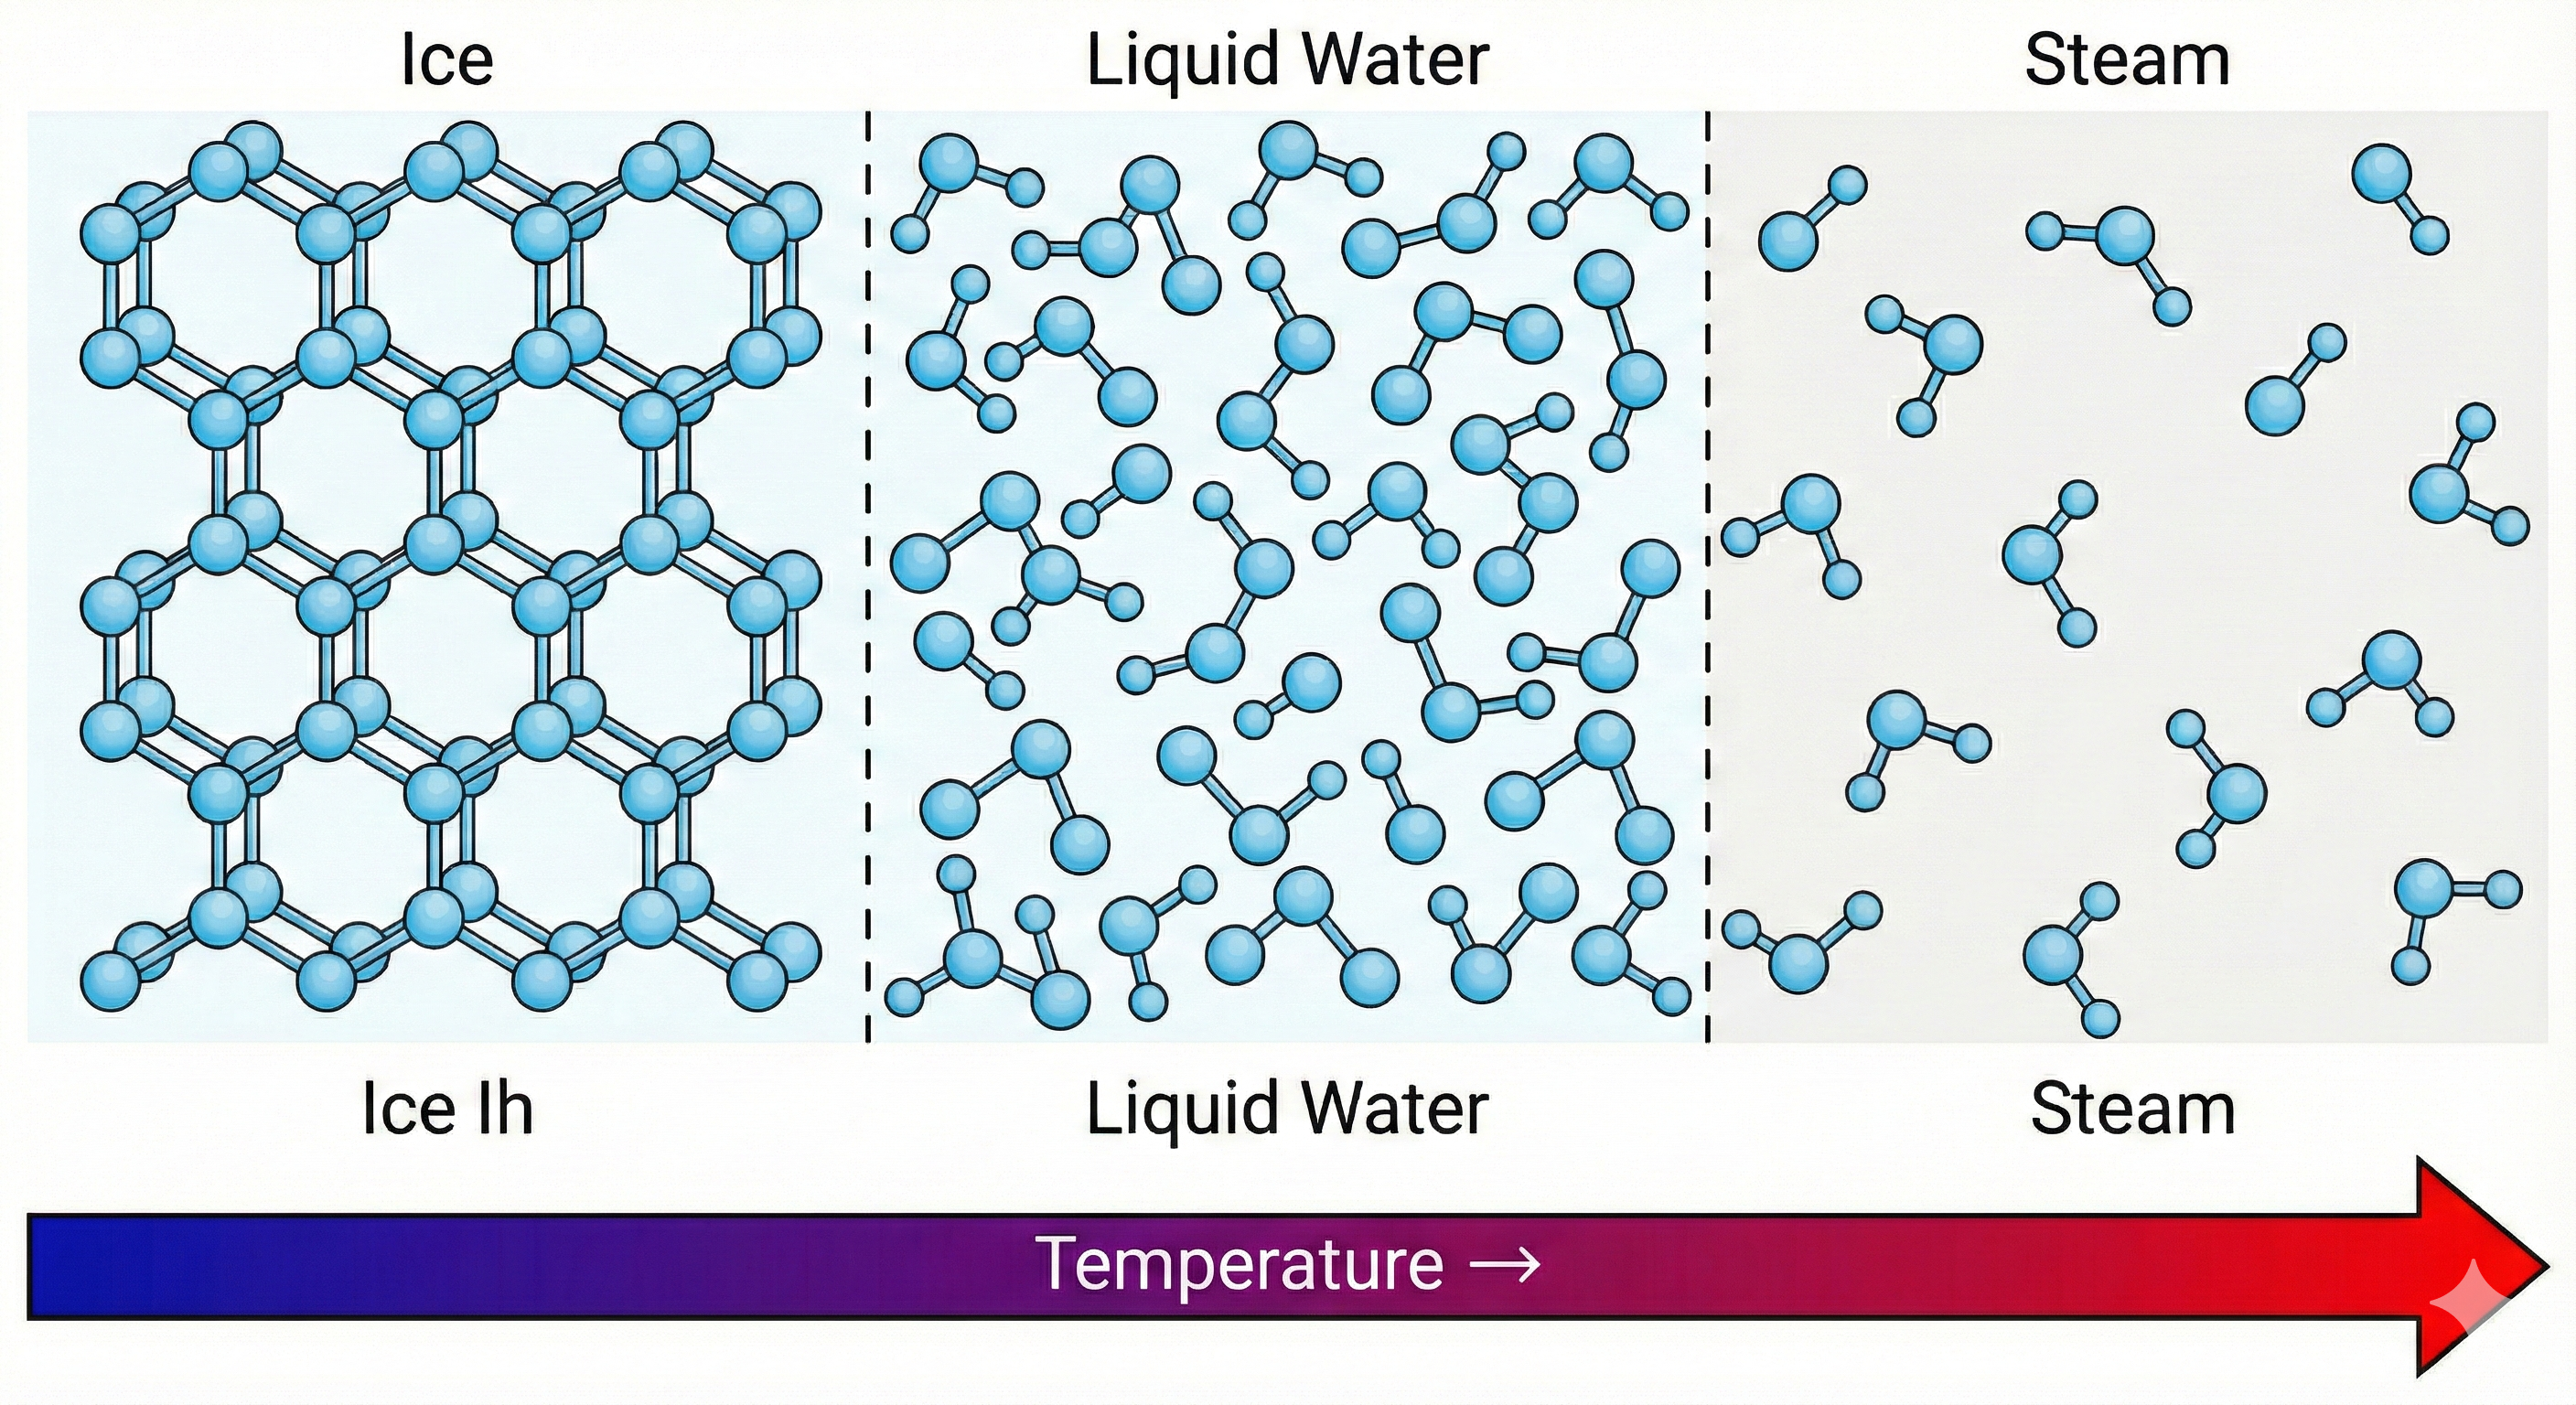
\includegraphics[width=0.85\textwidth]{figures/3.phase-transition.png}
\caption{Discrete phases without essences. The same H\textsubscript{2}O molecules constitute ice, liquid water, and steam; what differs is the collective behaviour at different temperatures. The boundaries between phases are sharp enough to skate on, swim in, and be shrouded by~-- yet no property intrinsic to the molecules makes them liquid rather than solid or gas. The discreteness is maintained by dynamics, not by essence.}
\label{fig:phase-transition}
\end{figure}

This is a model, not a metaphor. Language is not water. But the analogy opens conceptual space that the nominalist forecloses. If physical systems can exhibit discrete, stable, projectible structure without essences, so might linguistic ones. The question becomes empirical: what mechanisms play the role in language that thermodynamics plays for matter?

Consider a linguistic case where this shift pays off. Island constraints~-- configurations that resist extraction~-- seemed a paradigm of essentialist success. \textcite{ross1967} identified the patterns; subsequent decades spent refining the definition of an island (bounding nodes, barriers, phases). The definition kept shifting because the category refused to stabilize. \textcite{CuneoGoldberg2023Discourse} asked a different question. Not: what structural definition captures islands? But: what mechanism produces extraction resistance? Their answer: long-distance dependencies foreground a constituent, while certain constructions background their content. When functions clash, acceptability degrades. The mechanism explains the variable resistance without positing an essential island boundary.


\bigskip

Several traditions in linguistics have moved toward answers.

Usage-based approaches, developed by Joan Bybee and others, emphasize frequency and entrenchment \citep{bybee2010}. High-frequency patterns are stored with greater strength; they resist analogical change; they anchor categories. On this view, \mention{cattle} persists in its anomalous configuration because it is frequent enough to be learned as a unit rather than derived by rule.

Construction grammar treats form-meaning pairings as the basic units of grammar \citep{goldberg1995constructions}. Categories emerge from generalizations over constructions, not from innate specifications. Gradience is expected: novel uses inherit structure from prototypical uses, with acceptability shading off as similarity decreases~-- an outcome of acquisition, analogy, and the distribution of exemplars.

Sociolinguistics, from Labov onward, has documented that variation is orderly because transmission is orderly. The community maintains the system, and social dynamics shape what counts as grammatical where.

Functionalism grounds grammatical structure in communicative pressure. Categories persist because they do work: noun phrases package referents; tense locates events; definiteness manages discourse accessibility. When the pressure is strong, the clustering stabilizes; when it weakens, categories erode or restructure.

These traditions have the right instincts. They look for dynamics rather than definitions. They expect gradience and try to explain it. They treat stability as an achievement. But none has made mechanism fully central. Usage-based approaches invoke frequency; construction grammar invokes analogy; sociolinguistics invokes transmission. Recent work has begun to synthesize these insights \citep{schmid2020,spike2020,dahl2016}. What remains undeveloped is a systematic application to linguistic categories writ large, together with explicit diagnostic criteria.

That is the gap this book aims to fill.

\bigskip

Here is where the enterprise stalls.

If categories are maintained by mechanisms, then boundary cases become the most informative data, as Culicover \autocite*{culicover1999} argues in \textit{Syntactic Nuts}. They are where you can see the mechanisms at work, precisely because the mechanisms are under strain. But this requires criteria for failure. An account of what makes a category real needs a companion account of what makes a category \emph{not} real~-- a way to diagnose when the mechanisms are absent or insufficient. Without such criteria, mechanism-talk becomes unfalsifiable.

Chapter~\ref{ch:failure-modes} will develop these criteria in detail: the failure modes that distinguish genuine kinds from taxonomic conveniences. For now, the point is that the nominalist, having given up on essences, has also given up on the question of discipline. Haspelmath's comparative concepts are useful by stipulation; there is no further question of whether they carve at the joints. The mechanistic alternative promises something the nominalist abandons: a principled basis for saying that some categories are real and others are not, that some classifications reflect natural structure and others are artifacts of our methods.

But this promise depends on specifying what mechanisms do the maintaining. And that, in turn, depends on asking questions that neither tradition~-- essentialist nor nominalist~-- has posed.

\section{The lexeme obsession}
\label{sec:3:lexeme-obsession}

Return to the examples that opened this book: \mention{otherwise}, \mention{fun}, \mention{near}, \mention{cattle}. These are questions about items~-- about which box a particular word belongs in. They presuppose that the boxes exist.

The debate between essentialism and nominalism is, at bottom, a debate about these boxes. The essentialist says the boxes have necessary and sufficient conditions; the nominalist says they don't, and we should stop pretending otherwise. But both parties share an assumption: that the interesting ontological questions concern categories of \emph{lexemes}. Is \textsc{noun} a natural kind? Is \textsc{preposition}? Is \textsc{adjective} cross-linguistically real, or does each language have its own property-word category with no deep connection to any other?

This is the lexeme obsession. It has shaped the \emph{ontological} debate about categories for a century~-- the explicit discussion of natural kinds, essentialism, and prototype structure has overwhelmingly concerned parts of speech and constructions, not feature systems. The literature on noun-verb distinctions alone could fill a library. Every introductory syntax course spends weeks on parts of speech. Dissertations are written on whether a particular language has adjectives, or whether its property words are really a subclass of nouns or verbs. The question \enquote{what category is X?} is the bread and butter of descriptive linguistics.

Meanwhile, a different set of categories has received far less explicit ontological scrutiny~-- not because linguists haven't studied them, but because the metaphysical questions have rarely been made central.

\bigskip

What kind of thing is \textsc{gender}?

Not: which nouns are masculine, which are feminine, which are neuter. That's the lexeme question again~-- filing items into boxes. The question I'm asking is prior: what is the box itself? Is \textsc{gender} a natural kind, a feature of human grammars maintained by identifiable mechanisms? Or is it a label we apply to superficially similar systems that have no deep unity?

German gender and Swahili noun class both involve agreement. Both sort nouns into categories that condition the form of associated elements~-- articles, adjectives, verbs. Both are largely arbitrary from a semantic standpoint: German \mention{Mädchen} (girl) is neuter; Swahili \mention{kiti} (chair) is in a class that includes many artifacts but also trees. The similarities invite a common label. But Swahili has eighteen classes to German's three. Swahili classes are more semantically coherent in some cases, less in others. The agreement patterns differ in their syntactic domains. Are these the same kind of thing, or different things with a surface resemblance?

The generativist answer appeals to Universal Grammar: gender is a formal feature, part of the innate inventory of functional heads, realized differently across languages but unified at the level of underlying architecture. This is essentialism at the feature level~-- \textsc{gender} has an essence, even if individual gender systems vary in their particulars.

The typologist's answer, Haspelmath's answer, is that \textsc{gender} \emph{as a cross-linguistic category} is a comparative concept: a yardstick we construct for measuring diversity, with no claim to psychological reality in any particular speaker's grammar.

Neither answer asks what I want to know. What maintains gender systems? Why do languages have them at all? Why do they persist across generations, given that they're largely arbitrary and impose a significant learning burden? What functional or acquisitional or interactional pressures keep the clustering clustered?

\bigskip

The same questions arise for \textsc{number}.

English marks number with a suffix: \mention{cat}, \mention{cats}. The exponence is segmental, concatenative, largely predictable. A child who knows \mention{dog}/\mention{dogs} can produce \mention{wug}/\mention{wugs} \citep{berko1958}. The system is obligatory: you can't use a bare singular to refer to multiple cats. And it applies across the lexicon, with a handful of well-known exceptions (\mention{sheep}, \mention{deer}, \mention{cattle}). What English grammaticalizes is a distinction between singular and non-singular reference.

Shilluk, a Western Nilotic language spoken in South Sudan, also distinguishes singular from non-singular. But the exponence looks nothing like English. Shilluk marks number through stem-internal changes in tone, vowel length, and voice quality \citep{remijsen2019number}. The singular and plural of a noun may differ only in whether the vowel is short, long, or overlong~-- a three-way length distinction that exists in the lexical phonology but surfaces morphologically in number inflection. Or they may differ in tone: a Low singular becomes a Fall in the plural, or a Mid becomes a High. Or both. The patterns are largely unpredictable. A speaker who knows one singular-plural pair can't reliably derive another; each pair must be learned. Yet the system is obligatory in the same sense as English: nouns are specified for number, and that specification shows up in agreement.

\begin{table}[h]
\centering
\begin{tabular}{lll}
\textsc{singular} & \textsc{plural} & \textsc{gloss} \\
\hline
\ipa{yɪ̂t} & \ipa{yɪ́ːt} & `ear/ears' \\
\ipa{kàːl} & \ipa{káːl} & `fence/fences' \\
\ipa{pâːɲ} & \ipa{páːɲ} & `place/places' \\
\ipa{d̪âm} & \ipa{d̪áːm} & `blood (sg.)/bloods (pl.)' \\
\end{tabular}
\caption{Number marking in Shilluk: stem-internal changes (Remijsen \& Ayoker 2019)}
\label{tab:shilluk-number}
\end{table}

When we say that English and Shilluk both have number systems, what are we claiming they share? Not the exponence~-- one is affixal, the other fusional. Not the predictability~-- one is rule-governed, the other lexically specified. Not the phonological substance~-- one involves segments, the other suprasegmentals. What remains is something more abstract: both languages obligatorily distinguish singular from non-singular, and that distinction conditions agreement. Perhaps \textsc{number} is a natural kind after all~-- not at the level of morphological realization, but at the level of what the morphology is doing. Both systems, on this view, are grammatical reflexes of the same underlying operation: distinguishing individuated entities from pluralities.

Japanese suggests otherwise.

The noun \mention{hito} 人 means `person'. It can refer to one person or to multiple people; nothing in the grammar forces a choice. Where English requires \mention{person} or \mention{people}, Japanese allows \mention{hito} for both. There is a reduplicated form, \mention{hito-bito} 人々, but it does not mean simply `more than one person'. It has a collective or distributive flavour: `people as a group', `various people', `each of the people in question'. And it is not productively available across the lexicon. Some nouns reduplicate; most do not. The operation is lexically restricted in a way that English plural \mention{-s} is not.

Meanwhile, if you want to count people in Japanese, you use a numeral with a classifier: \mention{san-nin} 三人 `three people', where \mention{nin} 人 is the classifier for human beings. The individuation of bounded entities~-- the semantic core that was supposed to unify \textsc{number} cross-linguistically~-- is handled by the classifier system, not by morphology on the noun. The noun itself remains unspecified for number.

Typologists file \mention{hito-bito} under \textsc{number} nonetheless~-- calling it a plural, or a collective, or something in between \citep[cf.][]{baloglu2022,forza2016}. The disagreement is revealing. When we apply the vocabulary of number to Japanese, we are not sure what we are claiming.

So what do English, Shilluk, and Japanese share?

English and Shilluk both have obligatory singular/non-singular distinctions, realized by completely different morphological means. The semantic claim~-- that both track individuation~-- seems defensible. Japanese has optional, lexically restricted, semantically flavoured reduplication that does not straightforwardly mean `more than one', and a classifier system that handles the counting. If \textsc{number} is `grammatical encoding of individuation', then Japanese nouns do not have number; the classifiers do the work. But typologists describe \mention{hito-bito} as a number phenomenon. Are they wrong? Or is \textsc{number} a label we apply to a family of loosely related phenomena~-- obligatory affixation, unpredictable stem-internal changes, optional reduplication, classifier systems~-- that share a functional neighbourhood but not a common mechanism?

Definitional refinement cannot solve this. No set of necessary conditions will group obligatory affixation, lexically specified stem alternations, optional reduplication, and classifier systems in a way that tracks what typologists actually want to generalize about. The unity of \textsc{number}, if it exists, lies in the mechanisms that maintain these clusters: whether the same acquisitional, processing, and transmission pressures keep the relevant properties co-occurring, or whether we are simply filing convergent solutions under one convenient label. That is the empirical question.

There are important exceptions. Corbett's work on gender and number asks why these systems exist and what functions they serve \citep{corbett1991,corbett2000}. Bybee, Dahl, and the grammaticalization tradition treat tense-aspect-modality categories as emergent clusters maintained by usage patterns and diachronic pathways \citep{bybee1994,dahl1985}. Typological work on case, evidentiality, and person addresses similar questions. But this literature rarely frames its insights as a general metaphysics of features. The question \enquote{what kind of thing is \textsc{number}?} is usually implicit, answered in passing rather than posed directly.

\bigskip

\textsc{tense}. \textsc{aspect}. \textsc{mood}. \textsc{definiteness}. \textsc{person}. \textsc{case}.

Each of these is treated as a grammatical feature, a dimension along which languages vary, a parameter to be set or a category to be described. Each has generated an enormous literature. And for each, the explicit natural-kind question is usually background assumption rather than central topic.

Consider \textsc{definiteness}~-- a case I'll return to in detail in Chapter~\ref{ch:definiteness-and-deitality}. The textbook definition says that definite expressions pick out referents identifiable to the hearer. English \mention{the} is the paradigm case. But \mention{the} appears in contexts where identifiability fails: \mention{the hospital} in \mention{go to the hospital}, \mention{the tiger} in \mention{the tiger is endangered}, \mention{the average American} in statistical generalizations. Are these counterexamples to the definition, or extensions licensed by some deeper principle, or evidence that \textsc{definiteness} isn't a unified kind at all?

The usual move is to refine the definition: add accommodation, add familiarity, add uniqueness under a description. Each refinement handles some cases and strains on others. The definitional hunt continues.

The question I want to ask is different. What if \textsc{definiteness} and the form class that expresses it~-- the articles, the demonstratives, the possessives~-- are not one kind but two? The form side clusters by morphosyntactic properties: distribution, agreement, position. The meaning side clusters by semantic and pragmatic properties: identifiability, familiarity, specificity. These two clusters usually align. When they don't~-- the weak definites, the generic definites, the bridging cases~-- we see the seam between two distinct kinds, each maintained by its own mechanisms.

This is a different kind of question. It doesn't ask where to draw the boundary of \textsc{definiteness}. It asks whether \textsc{definiteness} is one thing or two, and what would tell us the difference.

\bigskip

The pattern should now be visible.

The essentialism-nominalism debate has focused on lexical categories: \textsc{noun}, \textsc{verb}, \textsc{adjective}, \textsc{preposition}. These are categories of items. The disputed cases are words~-- \mention{fun}, \mention{near}, \mention{otherwise}~-- and the question is which category they belong to.

But grammatical theory also posits categories of a different sort: features, dimensions, systems. \textsc{gender}, \textsc{number}, \textsc{tense}, \textsc{aspect}, \textsc{mood}, \textsc{definiteness}, \textsc{person}, \textsc{case}. These are not categories of items but categories of categories~-- ways of organizing the space in which items are located. A noun doesn't have a gender the way it has a phonological form. Gender is a system; the noun is assigned a value within that system.

These second-order categories have received surprisingly little ontological attention. We ask whether \textsc{noun} is a natural kind. We rarely ask whether \textsc{gender} is. We ask whether a particular language has adjectives. We rarely ask whether \textsc{tense} is a single phenomenon or a family of loosely related systems that share a label.

The reason, I suspect, is that features feel more abstract, more clearly theoretical, less tied to the messy particulars of words and constructions. Features are the machinery of the grammar, not the things the machinery operates on. It's natural to focus ontological scrutiny on the things~-- the lexemes, the constructions, the sentences~-- and treat the machinery as given.

But the machinery is exactly what needs scrutiny. If \textsc{noun} is a natural kind maintained by mechanisms, why not \textsc{gender}? If \textsc{preposition} is a cluster of properties that tend to co-occur, why not \textsc{tense}? If the question \enquote{is X a natural kind?} is worth asking for lexical categories, it's worth asking for feature systems too.

And once you ask it, you notice something.

Many central debates about feature systems are more radical than the usual lexical boundary disputes. The debate about whether \mention{fun} is a noun or an adjective is a boundary dispute: everyone agrees that \textsc{noun} and \textsc{adjective} exist; the question is where to draw the line between them. The debates about feature systems are more radical. They concern not where the boundaries fall but whether the categories exist at all.

Is \textsc{gender} a primitive, or is it reducible to NUMBER~-- a mechanism for individuation that enables counting? Some theorists have argued exactly this \citep{picallo1991,lowenstamm2008}. If they're right, then \textsc{gender} isn't a natural kind; it's a surface manifestation of NUMBER, and the apparent cross-linguistic diversity of gender systems is variation in how languages deploy individuation.

Is \textsc{tense} a primitive, or is it really a species of \textsc{aspect}~-- aspect anchored to the speech moment? If tense is just deixis applied to aspectual distinctions, then \textsc{tense} as a separate category dissolves. What we're left with is \textsc{aspect}, differently parametrized across languages.

Is \textsc{person} a primitive, or is it spatial deixis grammaticalized? First person as proximate, second person as distal, third person as remote? Some languages seem to work this way. If they all do, under the surface, then \textsc{person} is not a sui generis category but a special case of spatial orientation.

These are not boundary disputes. They're existential disputes. The question is not \enquote{where does \textsc{tense} end and \textsc{aspect} begin?} The question is whether \textsc{tense} exists as a distinct kind at all.

\bigskip

Neither essentialism nor nominalism naturally foregrounds these questions. The essentialist can revise the list of essences post hoc~-- \enquote{we were wrong; \textsc{tense} isn't basic after all}~-- but the framework provides no procedure for discovering reductions, only for registering them after the fact. The nominalist can note that some taxonomies are more useful than others, but treats the difference as pragmatic rather than as tracking structure in the world. A mechanistic approach asks what would settle the matter empirically.

What maintains \textsc{tense} as a distinct cluster? What maintains \textsc{aspect}? If they're maintained by the same mechanisms~-- if the properties that cluster as \enquote{tense} in one language are held together by the same forces that cluster as \enquote{aspect} in another~-- then the reduction is real, and \textsc{tense} is not a natural kind but a surface variant of something deeper. If they're maintained by different mechanisms, then both are real, and the apparent overlap is convergent evolution, not identity.

These are empirical questions. They have answers, even if we don't yet know what the answers are. The framework that makes them askable is the framework that treats categories as maintained by mechanisms, not constituted by essences.

\section{Grammaticality itself}
\label{sec:3:grammaticality}

There is one more question that neither tradition has posed, and it's the deepest.

Every analysis of every construction in every language presupposes a distinction between grammatical and ungrammatical sentences. The asterisk is the most common symbol in syntax. We mark \mention{*The cat slept the mat} as ungrammatical, \mention{The cat slept on the mat} as grammatical, and we build theories to explain the difference. The distinction is foundational. Without it, there's no data.

But what kind of thing is grammaticality?

The essentialist answer is that grammaticality is a property: a sentence either has it or doesn't. This picture faces well-known difficulties. Judgments are gradient; speakers disagree. The standard defense is the competence/performance distinction: the grammar is binary, the usage is messy. But if competence is a biological/cognitive state, we should not expect it to be captured by a tidy checklist of necessary properties. Biology is full of robust, stable kinds whose unity is maintained by interacting processes rather than fixed essences; if competence is real in that sense, homeostatic structure is the better default hypothesis than an all-or-nothing definition.

The prototype theorist's answer is that grammaticality is gradient. This captures the phenomenology but faces the same explanatory gap: if grammaticality is gradient, why is the gradient stable? Why don't judgments drift randomly?

Here is a question that almost no one asks: Is \textsc{grammaticality} itself a natural kind?

Not: is this sentence grammatical? That's the question we ask every day, the bread and butter of syntactic work. But: what kind of thing is the property we're probing when we ask that question? Is grammaticality a cluster of properties~-- acceptability, processability, learnability, attestation in corpora, consistency across speakers~-- held together by mechanisms? Or is it a single primitive, the output of an internalized grammar?

If it's a cluster, then the cases where the properties come apart~-- the sentences that are attested but judged unacceptable, or acceptable but never attested, or processable but not learnable~-- are evidence about the structure of the cluster. They reveal which mechanisms are doing which work.

If it's a primitive, then those cases are noise, or performance errors, or evidence that our elicitation methods are imperfect. The grammar is clean; the data are messy.

The choice between these views isn't a matter of taste. It's an empirical question about what grammaticality is and what maintains it. Chapter~\ref{ch:grammaticality-itself} will develop this question in detail. For now, the point is that grammaticality~-- the foundation of the entire enterprise~-- has received less ontological scrutiny than the categories it's used to define.

\section{What Part II provides}
\label{sec:3:what-part-ii-provides}

The questions raised in this chapter~-- what maintains \textsc{gender}? is \textsc{tense} a natural kind? what kind of thing is grammaticality?~-- can't be answered yet. To answer them, we need a framework that makes mechanism-talk precise: an account of what it is for a category to be maintained, what counts as a mechanism, how mechanisms interact, and how to tell when they're absent.

That's what Part II provides.

Chapter~\ref{ch:kinds-without-essences} introduces homeostatic property cluster kinds~-- the framework developed in philosophy of biology, here applied to linguistics. It specifies the mechanisms: acquisition, entrenchment, interactive alignment, iterated transmission, functional pressure. The chapter shows how they interact to produce the gradient structure that essentialism struggles with.

Chapter~\ref{ch:projectibility} asks what it takes for a category to support induction. Why can we generalize from observed nouns to unobserved ones? Why do the properties that cluster as \textsc{noun} predict further properties we haven't yet checked? The answer lies in the mechanisms: categories maintained by robust processes support inferences that arbitrary groupings don't.

Chapter~\ref{ch:failure-modes} develops the criteria for failure. When is a putative category too thin~-- too few properties, too weakly clustered? When is it too fat~-- multiple distinct kinds lumped under one label? When is it merely negative~-- a wastebasket category defined by what it's not? These diagnostics are what give the framework its teeth. They let us say, for particular cases, whether the mechanisms are sufficient to constitute a natural kind.

With that apparatus in place, Part III returns to the questions this chapter has raised. Chapter~\ref{ch:definiteness-and-deitality} takes up definiteness and argues that form and meaning constitute distinct but interacting kinds. Chapter~\ref{ch:lexical-categories} examines word classes~-- why nouns and verbs are stable across languages while adjectives and adverbs vary. Chapter~\ref{ch:the-stack} applies the framework across levels, from phonemes to constructions, showing that the same logic of clustering and maintenance applies at every scale. And Chapter~\ref{ch:grammaticality-itself} asks what we've deferred: what kind of thing grammaticality itself is, and what maintains it.

\bigskip

But first, the framework. The core idea is simple: categories are real because they are maintained. A noun is a noun not because it satisfies some checklist of necessary properties, but because the forces that cluster nominal properties~-- acquisition, frequency, analogy, transmission, function~-- keep clustering them.
